% Chapter Template

\chapter{Demostracion practicas} % Main chapter title

\label{Chapter5} % Change X to a consecutive number; for referencing this chapter elsewhere, use \ref{ChapterX}

%----------------------------------------------------------------------------------------
%	SECTION 1
%----------------------------------------------------------------------------------------
\section{P1: Pacman}
AL ser una aplicacion en el lado del servidor esta desarrolado  en JS. El usuario  abre el archivo 'gamePacman.html' dando lugar a la interpretacion del archivo por el navegador. En este punto se muestra el scenario de juego con todos los elementos cargados (pacman,fantasmas,cocos y obtaculos) \ref{fig:InitGame}. Disponemos  de un panel informativo sobre datos de la partida como el cronometro,numero de vidas,numero de cocos comido.
\begin{figure}[!h]
\centering
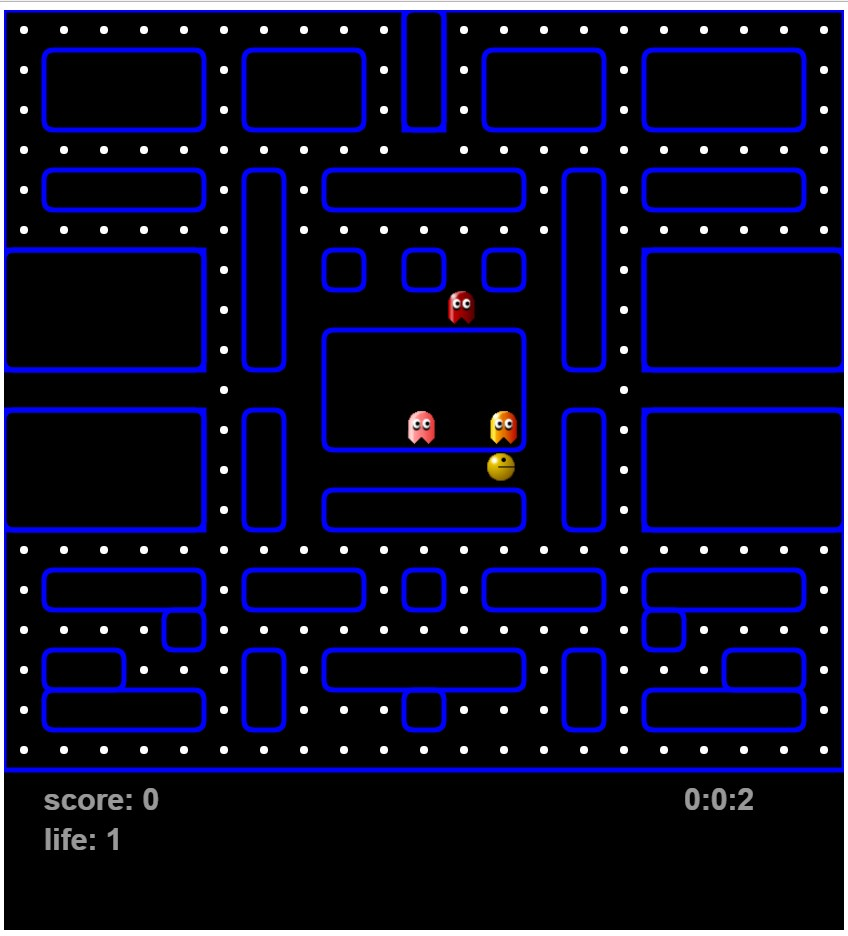
\includegraphics[width=43mm]{Figures/InitGame}
\decoRule
\caption[Inicio Juego]{Inicio juego Pacman.}
\label{fig:InitGame}
\end{figure}
\\El usuario por motivos externos al juego puede querer parar la partida que lo puede realizar pulsando la tecla 'P' y para volver a a la patida solo tiene que pulsar la tecla 'L'.\ref{fig:Pause/Start game}
\begin{figure}[htbp]
\centering
\subfigure[Juego pausado]{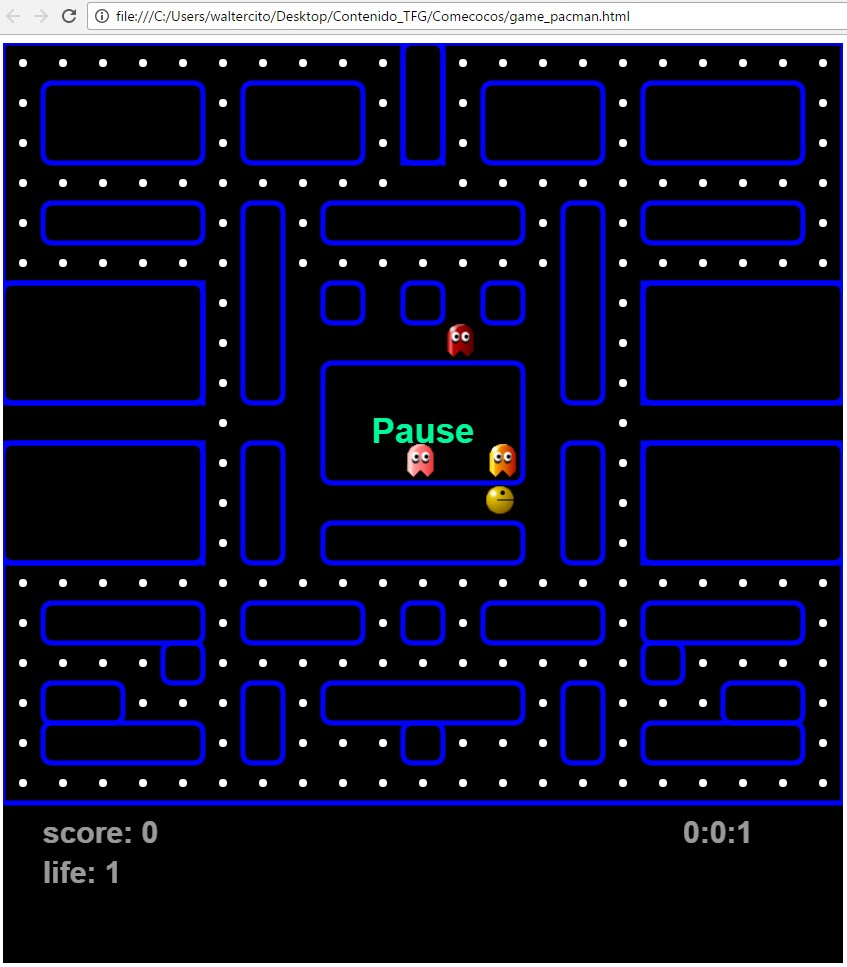
\includegraphics[width=40mm]{./PauseGame}}\hspace{5mm}
\subfigure[Juego no pausado]{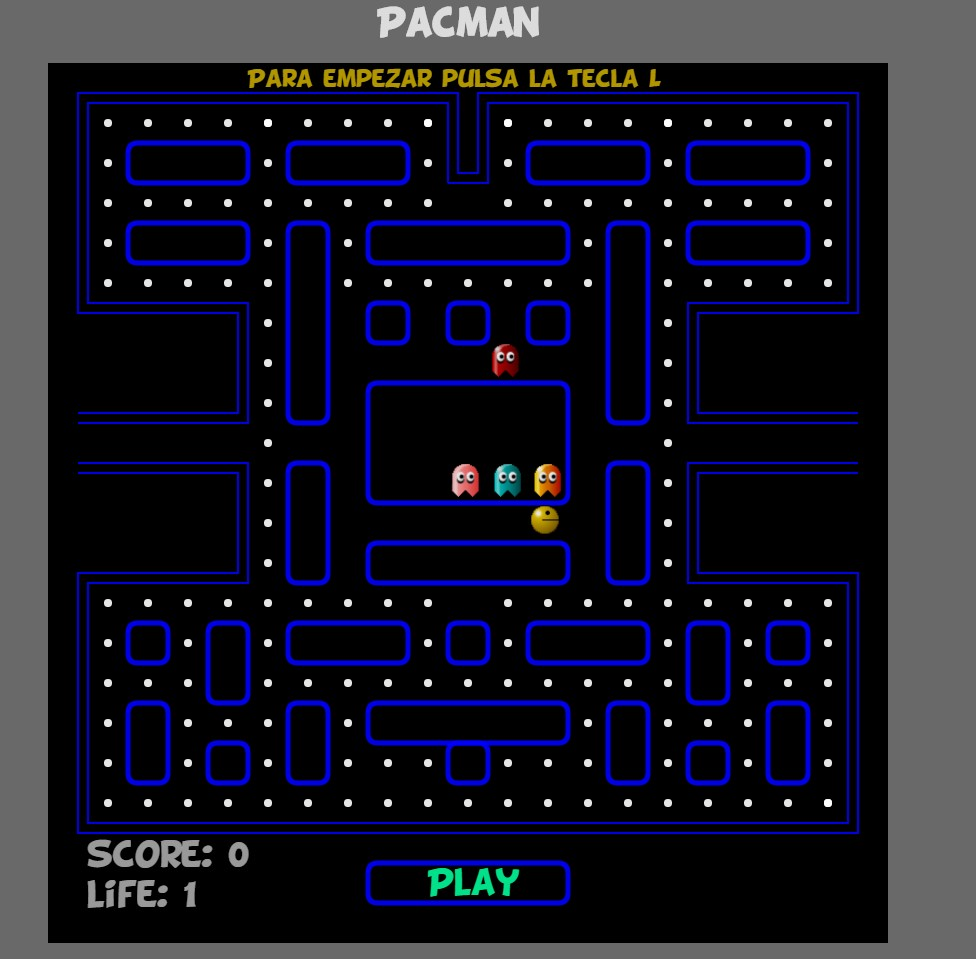
\includegraphics[width=40mm]{./InitGame}}
\caption{Pause/Start juego.} \label{fig:Pause/Start game}
\end{figure}
\\La partida termina en dos posibles casos \ref{fig:Game/Loose game}
\begin{enumerate}
\item Cuando uno de los fantasmas atrapa a Pacman daremos la partida como perdida y en la pantalla se visualiza 'Game Over'.
\item Cuando Pacman se ha comido todos los cocos de la partida finaliza la partida ya que el usuario ha ganado la partida. El usuario visualiza 'Win Game' y si quiere guardar informacion de la partida puede pulsar 'Save Score'.
\end{enumerate}
\begin{figure}[htbp]
\centering
\subfigure[Partida perdida]{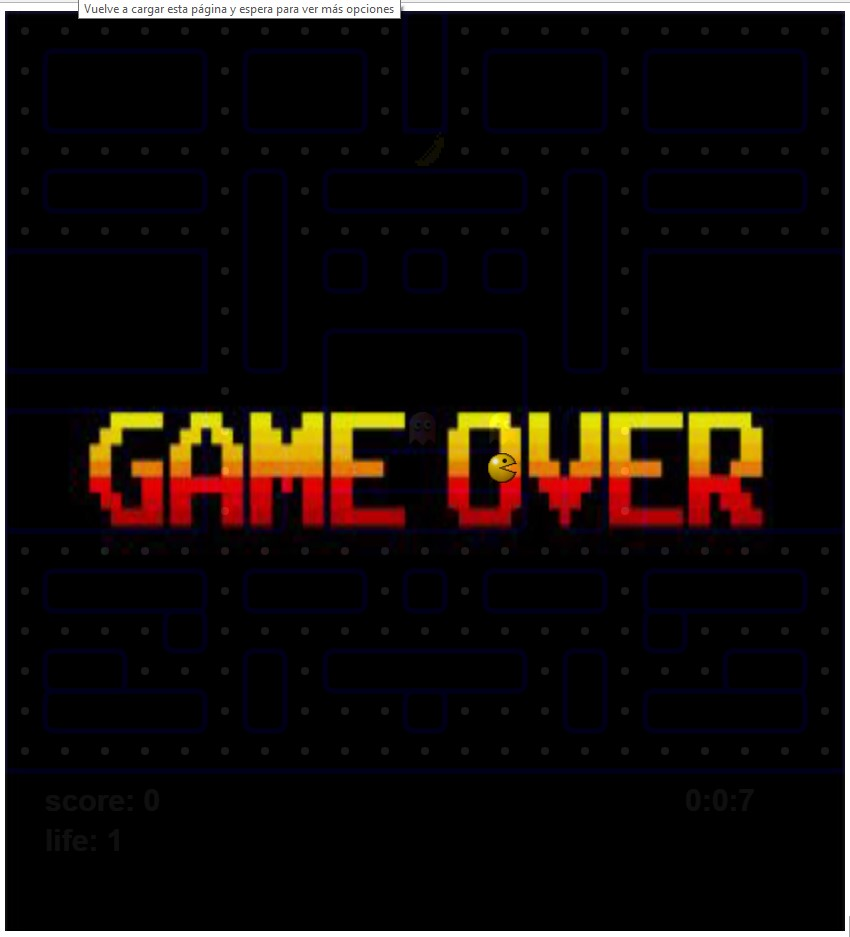
\includegraphics[width=40mm]{./GameOver}}
\subfigure[Partida Ganada]{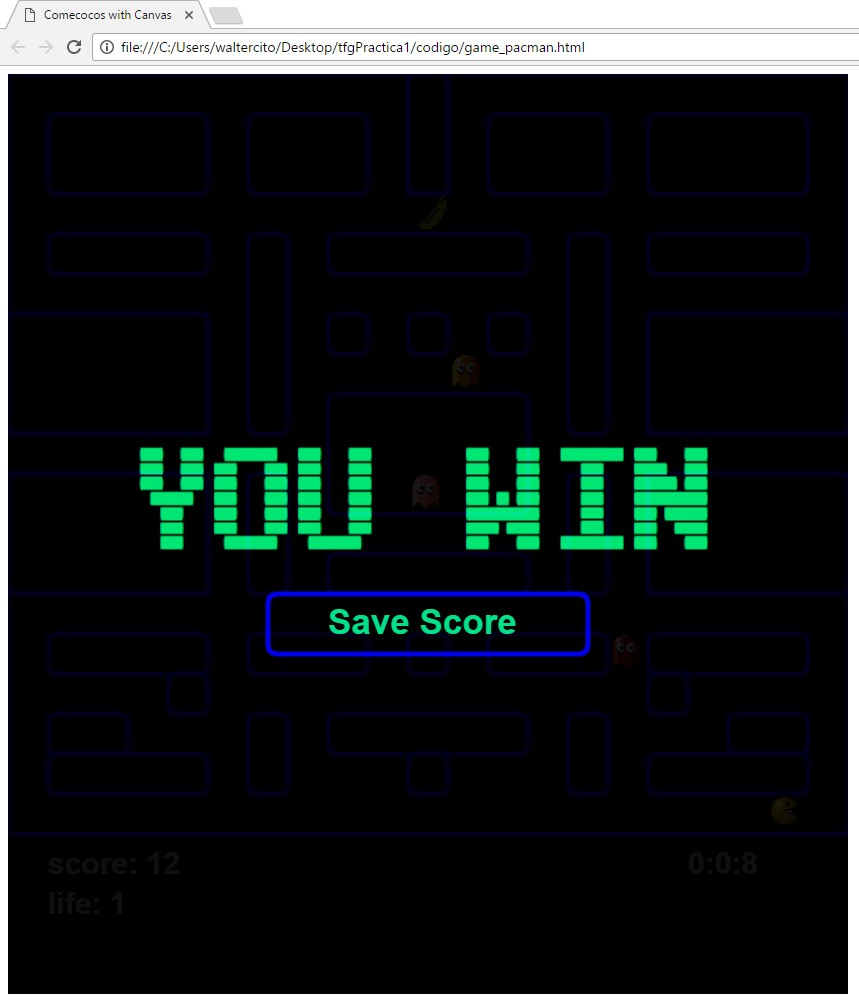
\includegraphics[width=40mm]{./Win_Game}}
\caption{Game/Loose juego.} \label{fig:Game/Loose game}
\end{figure}
%----------------------------------------------------------------------------------------
%	SECTION 2
%----------------------------------------------------------------------------------------
\section{P2: Pacman-Online}
%----------------------------------------------------------------------------------------
%	SECTION 2
%----------------------------------------------------------------------------------------
\section{P3: Desarrollo pagina web}
Lanzamos el servidor de la aplicacion llamando por consola 'python runserver'
el cual se lanza en la  direccion '127.0.0.1:8181'.
%-----------------------------------
%	SUBSECTION 1
%-----------------------------------
\subsection{Admin Django}
Accedemos al Admin del proyecto en el que podemos ver cada uno de los modelos que se han utilizado para el desarrollo de la practica , como mensionamos en el capitulo 3.3.


\subsection{Visualizacion Ventanas}
Ahora pasamos a visitar el sitio web para ello introducimos en el navegador la siguiente url 'http://127.0.0.1:8181/recursos/' en la que se recarga la pagina principal de la web. ref[img]
\\A traves del toolbar accedemos a las distintas paginas de la web como son festivales, artistas, imagenes y videos a traves del desplegable que se genera al pulsar en una de las opciones anteriores. ref[imagenes ventanas]

%-----------------------------------
%	SUBSECTION 2
%-----------------------------------
\subsection{Gestion Usuarios}
Hasta el momento hemos visualizado los elementos de la pagina web ahora pasamos a la gestion  de usuarios. Para ello el usuario tiene dos opciones , la primera es registrarse en la web ,ref 5.3  o hacer login siempre que el usuario se haya registrado previamente, ref 5.3.

Cuando el usuario ha entrado en el sitio web con sus credenciales se habilita la opcion 'perfil' en el cual puede modificar sus datos o simplemente realizar una consulta de los mismos, ref 5.4

En cuanto a la modificacion del perfil con esta opcion el usuario puede modificar los datos  y la imagen asociado ya que en la creacion del perfil se coloca una imagen por defecto. ref 5.5
%-----------------------------------
%	SUBSECTION 3
%-----------------------------------
\subsection{Formulario}
Cuando el usuario necesite hacer una consulta/queja sobre el servicio prestado por la Web o si necesita conocer informacion sobre algun elemento que no ha encontrado.Para esto dispone de la opcion 'Contacta' que presenta un formulario para que el usuario lo rellene segun sus necesidades. ref [IMG Contacta]
%-----------------------------------
%	SUBSECTION 4
%-----------------------------------
\subsection{Buscador}
Los usuarios disponen de una barra de busqueda a traves de la cual el usuario puede introducir el nombre del elemento que necesite consultar.Si el elemento que se busca existe  se muestra un deplegable con la informacion en caso contrario no se muestra nada.\ref{fig:Buscador web}
\begin{figure}[htbp]
\centering
\subfigure[Arya y Reeds]{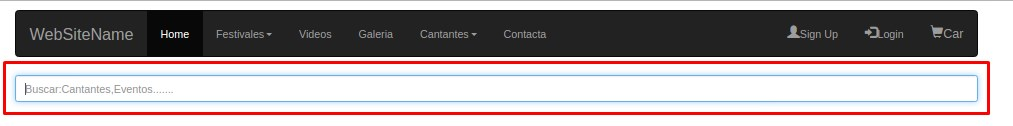
\includegraphics[width=80mm]{./Buscador}}
\subfigure[Lannisters]{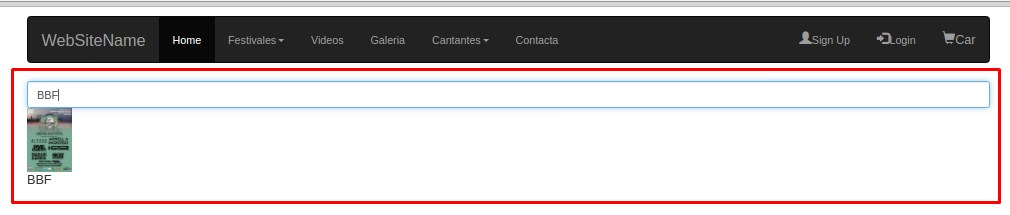
\includegraphics[width=80mm]{./ResultSearch}}
\caption{Buscador web.} \label{fig:Buscador web}
\end{figure}
%-----------------------------------
%	SUBSECTION 5
%-----------------------------------
\subsection{Carrito compra}
El usuario añade el contenido al carrito de la compra cuando necesite comprar entradas para un festival por ejemplo. A traves del icono del carrito se consulta el contenido que el usuario ha añadido y tiene la opcion de realizar la compra del contenido pulsando en el boton 'buy'. ref[Img Car]
\\Una vez, realizada la compro los productos  aparecen en el perfil del usuario. [Img PerfilModif]


\section{P4: Multi-chat Peer-to-Peer}
Para las pruebas que vamos a exponer el navegador que se ha utilizado es Mozilla Firefox ya que los otros navegadores presentan mecanimos de seguridad que impiden conexiones no seguras con webSockets.
\\Primero  lanzamos el servidor de señalizacion el cual se encuentra en una direccion publica para tener acceso , para nuestras pruebas se ha utilizado la IP publica del los laboratorios de robotica de la universidad.  ref.5.4.1
\\Los usuarios se conectan a la direccion  'IP:Puerto' dando acceso a la aplicacion la cual pedira el  nombre de usuario que se utilizara durante las conexiones.Dentro de la aplicación el usuario debe seleccionar el contenido que desee compartir (audio y/o video)  y la forma de la que desea hacerlo ya sea a traves de una sala existente o una nueva que el usuario creara .\ref{fig:Interaccion}( a)
\begin{figure}[htbp]
\centering
\subfigure[Seleccion Sala]{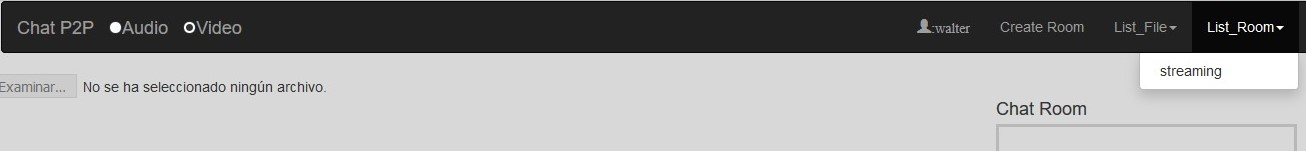
\includegraphics[width=65mm]{./SelectRoom}}\hspace{5mm}
\subfigure[Peticion conectar elementos]{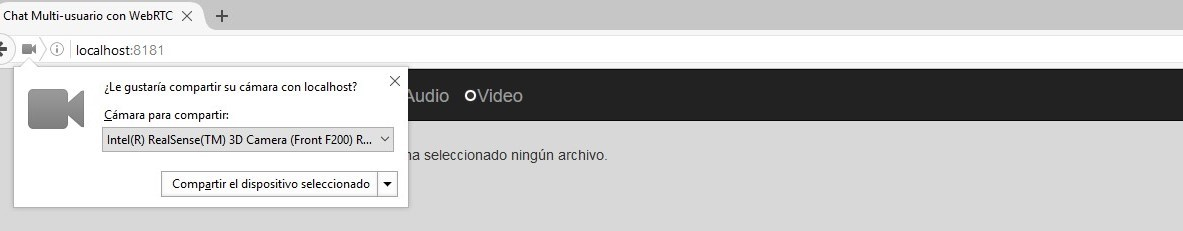
\includegraphics[width=65mm]{./peticionElementos}}
%\subfigure[Visualizacion elementos locales]{\includegraphics[width=80mm]{./Coneccion}}
\caption{Interaccion .} \label{fig:Interaccion}
\end{figure}
\\Tras seleccionar los elementos anteriores se envia el mensaje de conexion al servidor el cual envia un mensaje permitiendo el acceso a la sala y la conexion de los elementos seleccionados.El usuario puede o no aceptar compartir los elemento ,\ref{fig:Interaccion}(b) .En caso afirmativo el usuario visualiza el contenido de la web cam y microfono aun que el chat permanece inactivo ya que el usuario se encuentra solo en la sala. \ref{fig:ConnectElementLocal}
\begin{figure}[!h]
\centering
\includegraphics[width=0.8\linewidth]{Figures/Coneccion}
\decoRule
\caption[An Electron]{Conexion elementos locales.}
\label{fig:ConnectElementLocal}
\end{figure}
A medida que otros usuarios se unan a la sala  se añade el contenido de sus webcams en la parte inferior de la web.En este momento el chat esta disponible al igual que el input a traves el cual podemos enviar un fichero a todos los usuarios de la sala. ref.4.3
El proceso de la conexion se basa en WebRTC y la utilizacion de sus API quienes permiten  establecer la comunicacion entre varios nodos.A continuacion pasamos a demostrar el comportamiento de la aplicacion en distintos escenario centrandonos en el protocolo ICE el cual se encarga de obtener la informacion de la red pero funciona de distinta dependiendo de la configuracion que presente por lo que con ayuda del Wireshark verificaremos este comportamiento.
\subsection{Conexión en redes distintas}
Cuando trabajamos con el protocolo ICE , este es el encargado de obtener la informacion de red en la que el nodo esta ejecutando la aplicacion.
\subsubsection{Implementacion con STUN}
Como se explico en el capituo 3 , cuando intentamos conocer

\subsubsection{Implementacion con TURN}
